\documentclass[preprint,12pt,authoryear]{elsarticle}

\usepackage{amssymb}
\usepackage{amsmath}
\usepackage{graphicx}
\usepackage{subcaption}
\usepackage{booktabs}
\usepackage{tikz}
\usetikzlibrary{positioning}

\journal{Advances in Space Research}

\begin{document}

\begin{frontmatter}

\title{Discrete Element Modeling of Lunar Regolith Tribocharging in Vibratory Feeders under Reduced Gravity using LIGGGHTS}

\author[1]{Tejas R}
\ead{tejasr.me@rvce.edu.in}

\author[1]{Dr. Nanjundaradhya N V\corref{cor1}}
\ead{nanjundaradhya@rvce.edu.in}
\cortext[cor1]{Corresponding author}

\affiliation[1]{organization={Department of Mechanical Engineering, RV College of Engineering},
            addressline={Mysore Road, RV Vidyaniketan Post}, 
            city={Bengaluru},
            postcode={560059}, 
            state={Karnataka},
            country={India}}

A sustained human presence on the Moon requires the local extraction and processing of resources, yet dry electrostatic beneficiation of lunar regolith remains a critical, low-TRL bottleneck due to flow jamming and severe charge-to-mass ratio attenuation under reduced gravity. Here, we present a coupled Discrete Element Method (DEM) and energy-based triboelectric contact-electrification model that uncovers the micro-mechanical origins of this bottleneck. By calibrating the Hertz-Mindlin contact model with SJKR cohesion against the experimental angle of repose of the LMS-1 lunar simulant, we show that the six-fold gravity reduction shifts the granular assembly into a high Granular Bond number regime ($Bo_g \approx 8.04$), prompting a gravity-dependent transition to a cohesion-dominated jammed state. We demonstrate that lunar gravity dampens relative impact velocities, triggering a severe 67\% reduction in charge acquisition (to 0.16 $\mu$C/g) under lunar gravity at a standard 1.0 mm amplitude compared to the terrestrial baseline (0.50 $\mu$C/g). While terrestrial vibratory transport successfully operates at 1.0 mm amplitude, lunar feeders require a doubling of mechanical vibration intensity ($\ge 2.0$ mm amplitude) to achieve fluidization and recover a charge-to-mass ratio of 0.51 $\mu$C/g, satisfying the baseline dry beneficiation target. Our findings establish quantitative physics-based guidelines for next-generation planetary feed mechanisms, proving that high-intensity vibratory regimes ($\ge 2.0$ mm) are required to overcome gravitational velocity damping and enable viable resource beneficiation on the Moon.


\begin{keyword}
Lunar regolith \sep DEM simulation \sep ISRU \sep Granular Bond number \sep Triboelectric charging \sep Vibratory feeder
\end{keyword}

\end{frontmatter}

\section{Introduction}
\label{sec:intro}

The long-term sustainability of crewed lunar exploration relies on In-Situ Resource Utilization (ISRU)---the extraction of oxygen, water, and structural metals from local regolith \citep{ISECG2021, Li2018}. Within the ISRU value chain, beneficiation, which involves the mechanical sizing, sorting, and mineral enrichment of raw regolith prior to chemical reduction, remains a critical bottleneck, currently assessed at Technology Readiness Level (TRL) 3--4. Dry electrostatic separation exploits the differential triboelectric charging of mineral grains based on their dielectric properties. It is considered a leading candidate for lunar dry beneficiation to concentrate target minerals such as ilmenite (FeTiO$_3$) in waterless environments \citep{Trigwell2009, Trigwell2006, Trigwell2007}.

The effectiveness of electrostatic separators is fundamentally governed by the feed mechanism, which transports regolith into the separation field while inducing a differential tribocharge through controlled particle-wall collisions \citep{Franke2024}. Current terrestrial systems typically employ passive, gravity-fed mechanisms, including free-fall chutes and static mixer baffles. In the lunar environment, however, these passive systems face dual failure modes: insufficient particle collision energy to generate the minimum charge-to-mass ratio ($Q/M$) required for separation \citep{Trigwell2009}, and mechanical blockage caused by the cohesion-dominated flow behavior of fine lunar regolith \citep{Colwell2007, Taylor2010}.

Understanding the flow of granular media under varying gravitational conditions is critical to designing robust handling systems \citep{Murdoch2013, Murdoch2012}. The transition from free-flowing to jamming behavior can be theoretically framed using the Granular Bond Number ($Bo_g$), which compares cohesive inter-particle forces against the material's weight \citep{Madden2025, Scheeres2010}. On Earth, the weight of a typical regolith particle dominates cohesion ($Bo_g < 1$), leading to a steady, gravity-driven flow. Under lunar gravity (1.62 m/s$^2$), the gravitational force is reduced by a factor of six, while the material-specific cohesive forces remain constant. For fine particles, particularly those smaller than 200 $\mu$m, this shifts the balance such that $Bo_g > 1$, signaling a transition to a cohesion-dominated regime where particles clump and jam in passive geometries \citep{Hartzell2011, Scheeres2010}. Active vibratory feed mechanisms are therefore required to supply mechanical energy to overcome this cohesive threshold \citep{Richards2004}.

There remains a critical need to computationally quantify how the vibration parameters (frequency and amplitude) of an active feeder must be retuned specifically for the lunar gravity environment to overcome regolith cohesion and maximize triboelectric charge acquisition. Existing DEM models for charged granular media \citep{Galvin2021, Wu2020} have not been applied to a vibratory feeder operating under reduced gravity conditions coupling an SJKR cohesion model with a collision energy charging model ($Q = f(E)$). While particle-size dependent bipolar charging is documented \citep{Forward2009}, numerical studies isolating the fundamental energy transfer are needed to guide prototype development. 

This study outlines a coupled DEM and tribocharging methodology with the following objectives: (1) calibrate the SJKR cohesion coefficient in DEM to match the physical angle of repose of LMS-1 lunar simulant; (2) formulate and implement a $Q = f(E_{\mathrm{collision}})$ charge transfer model as a post-processing application; and (3) conduct parametric DEM simulations across different vibration amplitudes and gravity levels to quantify the relationship between vibration, mass flow, coordination number, and charge accumulation. The rest of the paper is organized as follows: Section 2 details the computational contact mechanics, calibration protocols, and simulation setup; Section 3 presents the granular fluidization, impact kinetics, and parametric charging results; Section 4 provides a deep discussion on coarse-graining limits, engineering design guidelines, and the full-scale calibration roadmap; and Section 5 summarizes the conclusions.

\section{Methodology}
\label{sec:method}

The computational methodology integrates a DEM simulation framework to resolve the granular flow dynamics with a Python-based post-processing architecture to quantify triboelectric charge acquisition. This computational pipeline is structured in three sequential, interdependent phases:
\begin{enumerate}
    \item \textbf{Phase 1 (Cohesion Calibration):} A cylinder-lift Angle of Repose (AoR) test is simulated under Earth gravity. The SJKR cohesion energy density $k_c$ is iteratively swept and calibrated until the heap slope matches the physical LMS-1 regolith simulant benchmark ($38.3^\circ \pm 2^\circ$).
    \item \textbf{Phase 2 (Charging Calibration):} The material properties are locked. A terrestrial simulation is run on a flat-plate vibratory feeder at $1.0\text{ mm}$ amplitude and $40\text{ Hz}$. The post-processing charge transfer coefficient $k_d$ is calibrated such that the terminal charge converges to $0.50\ \mu\text{C/g}$, matching the experimental Trigwell benchmark.
    \item \textbf{Phase 3 (Parametric Production Sweeps):} The fully calibrated granular digital twin is subjected to a parametric sweep crossing Earth and Moon gravities and three vibration amplitudes ($0.5\text{ mm}$, $1.0\text{ mm}$, $2.0\text{ mm}$) at a fixed $40\text{ Hz}$ frequency, generating a comprehensive charging and fluidization performance matrix.
\end{enumerate}

\subsection{DEM Simulation Framework}
\label{sec:dem_framework}
Simulations of the granular flow within the vibratory feeder were performed using the open-source DEM code LIGGGHTS \citep{Kloss2012, Hager2014}. The solver explicitly tracks the position, velocity, and collision dynamics of individual particles across discrete timesteps using parallelized algorithms \citep{Plimpton1995}. To prevent silent-crash failure modes, the methodology was split into a sequential validation pipeline: analytical property calibration, toolchain verification using simple geometries, and finally, the parametric study in the full prototype geometry.

\subsection{Contact Model: Hertz-Mindlin with SJKR Cohesion}
To capture the cohesive nature of lunar regolith, the contact dynamics were modeled using the Hertz-Mindlin contact formulation \citep{DiRenzo2004, Mindlin1949} augmented with the Simplified Johnson-Kendall-Roberts (SJKR) cohesion model \citep{Johnson1971}. The Hertz-Mindlin model resolves the normal and tangential repulsive elastic forces and viscous damping during a collision. The normal contact force ($F_n$) is written as:
\begin{equation}
F_n = \frac{4}{3} Y^* \sqrt{R^*} \delta_n^{3/2} - 2 \sqrt{\frac{5}{6}} \beta \sqrt{S_n m^*} v_{n,\mathrm{rel}}
\end{equation}
where $Y^*$ and $R^*$ are the equivalent Young's modulus and radius, $\delta_n$ is the normal overlap, $v_{n,\mathrm{rel}}$ is the relative normal velocity, $m^*$ is the equivalent mass, $\beta$ is the viscoelastic damping coefficient, and $S_n = 2 Y^* \sqrt{R^* \delta_n}$ is the normal contact stiffness.

Similarly, the tangential force ($F_t$), limited by the Coulomb friction limit ($\mu_s F_n$), is formulated as:
\begin{equation}
F_t = -8 G^* \sqrt{R^* \delta_n} \delta_t - 2 \sqrt{\frac{5}{6}} \beta \sqrt{S_t m^*} v_{t,\mathrm{rel}}
\end{equation}
where $G^*$ is the equivalent shear modulus, $\delta_t$ is the tangential displacement, $v_{t,\mathrm{rel}}$ is the relative tangential velocity, and $S_t = 8 G^* \sqrt{R^* \delta_n}$ is the tangential contact stiffness.

The SJKR model adds a constant attractive cohesive force ($F_c$) proportional to the particle contact area, independent of the deformation history \citep{Roessler2018}:
\begin{equation}
F_{c} = -k_{c} A
\end{equation}
where $k_{c}$ is the cohesion energy density (J/m$^3$) and $A = \pi (R^* \delta_n)$ is the contact area. This parameter acts as the primary material property defining the cohesion of the simulant.

\subsection{Material Properties and Scaling Rationale}
The simulated granular material properties were mapped to the Lunar Mare Simulant-1 (LMS-1), a standard high-fidelity lunar simulant designed to represent the physical and mineralogical characteristics of Apollo mare soils \citep{Britt2019}. A uniform particle diameter of 1.0 mm and a particle density of 2920 kg/m$^3$ were adopted. To permit a numerically stable and practical timestep, the Young's modulus of the particles was scaled down from the physical value of $\sim$60 GPa to 20 MPa. This soft-sphere scaling approach is a standard practice in granular DEM literature \citep{Roessler2018, Coetzee2017}, ensuring that the integration timestep remains below the critical Rayleigh limit without artificially altering the macroscopic flow behavior. While the softer particles experience extended contact durations, the macroscopic kinetic energy field—which drives the tribocharging model—is statistically preserved because the coefficient of restitution ($e=0.5$) dictates the consistent energy dissipation per collision. 

A constant rolling friction of 0.1 and sliding friction of 0.5 were applied across all runs. Furthermore, because the lunar beneficiation environment is a hard vacuum, aerodynamic drag forces are physically zero. Consequently, standalone DEM (without CFD coupling) is the physically accurate framework for modeling lunar particle transport \citep{Brodu2015}. The complete set of macroscopic material parameters and calibrated contact properties used across all simulations is summarized in Table \ref{tab:material_properties}.

\begin{table}[htbp]
\centering
\caption{DEM Simulation Parameters for LMS-1 Lunar Simulant}
\vspace{0.15cm}
\label{tab:material_properties}
\resizebox{\textwidth}{!}{
\begin{tabular}{lll}
\toprule
\textbf{Parameter} & \textbf{Value} & \textbf{Remarks} \\ \midrule
Particle Diameter ($d$) & 1.0 mm & Scaled for computational efficiency \\
Particle Density ($\rho$) & 2920 kg/m$^3$ & Physical LMS-1 property \citep{Britt2019} \\
Young's Modulus ($Y$) & 20 MPa & Soft-sphere scaled \citep{Coetzee2017} \\
Poisson's Ratio ($\nu$) & 0.25 & Standard silicate assumption \\
Coefficient of Restitution ($e$) & 0.5 & Particle-Particle / Particle-Wall \\
Sliding Friction ($\mu_s$) & 0.5 & Baseline friction \\
Rolling Friction ($\mu_r$) & 0.1 & Baseline rolling resistance \\
SJKR Cohesion Density ($k_c$) & 285,000 J/m$^3$ & Calibrated to 38.3$^\circ$ AoR \\
Integration Timestep ($\Delta t$) & $5 \times 10^{-7}$ s & $< 10\%$ of Rayleigh time \\ \bottomrule
\end{tabular}
}
\end{table}

\subsection{Angle of Repose Calibration Protocol}
Because $k_c$ is a macroscopic contact-scale proxy parameter rather than a directly measurable physical constant, it must be calibrated empirically \citep{Coetzee2017, Lommen2014}. We implemented a simulated cylinder-lift test under Earth gravity ($9.81\text{ m/s}^2$): particles are settled inside a cylinder of diameter $40\text{ mm}$ and allowed to decay to complete hydrostatic equilibrium. The cylinder is then lifted vertically along the Z-axis at $0.05\text{ m/s}$ to a height of $50\text{ mm}$, letting the column collapse under gravity to form a stable, cohesive, conical pile.

To eliminate subjective error, a mathematical pile-profiling algorithm extracts a cross-sectional slice of the pile, maps the surface boundary peaks, and uses linear regression to fit the left and right slopes. The repose angle ($\theta$) is then computed as $\theta = \arctan(|m|)$ (where $m$ is the slope gradient).

Critically, this empirical calibration method inherently justifies the use of scaled 1.0 mm particles instead of physical 91 $\mu$m grains. Since coarse-graining scales up the grain diameter from $91\ \mu\mathrm{m}$ to $1.0\text{ mm}$, the cohesion energy density $k_c$ must be scaled up by an analytical scaling factor of approximately $10.99$ to preserve the dimensionless Granular Bond Number ($Bo_g$) \citep{Roessler2018}. This guarantees that the simulated fluidization and flow mechanics maintain dynamic similarity to the physical powder.

To identify the correct cohesion energy density $k_c$, we executed an iterative calibration sweep at a fast-run population of $N = 5,000$ particles, starting from a low cohesion energy density of $50,000\text{ J/m}^3$ and scaling up until the simulated repose angle matched the physical target repose angle of LMS-1 ($38.3^\circ \pm 2^\circ$) \citep{Carrier1991}. The results of these iterations are summarized in Table~\ref{tab:paper_calibration_iterations}.

\begin{table}[htbp]
    \centering
    \caption{Cohesion calibration iteration sweep history for LMS-1 simulant.}
    \label{tab:paper_calibration_iterations}
    \resizebox{\textwidth}{!}{
    \begin{tabular}{cccccp{6cm}}
        \hline
        \textbf{Iteration} & \textbf{Particle Count} & \textbf{Cohesion ($k_c$)} & \textbf{Simulated AoR} & \textbf{Target AoR} & \textbf{Notes} \\ \hline
        v1 & 5,000 & $50,000\text{ J/m}^3$ & $22.4^\circ$ & $38.3^\circ \pm 2^\circ$ & Cohesion highly insufficient; heap is flat. \\
        v3 & 5,000 & $150,000\text{ J/m}^3$ & $29.8^\circ$ & $38.3^\circ \pm 2^\circ$ & Partially cohesive behavior; angle remains too low. \\
        v5 & 5,000 & $250,000\text{ J/m}^3$ & $35.1^\circ$ & $38.3^\circ \pm 2^\circ$ & Approaching experimental bounds. \\
        v7 & 5,000 & $285,000\text{ J/m}^3$ & $37.9^\circ$ & $38.3^\circ \pm 2^\circ$ & Within experimental tolerance. Fast sweep converged. \\
        \textbf{v8 (Final)} & \textbf{20,000} & \textbf{$285,000\text{ J/m}^3$} & \textbf{$38.6^\circ$} & \textbf{$38.3^\circ \pm 2^\circ$} & Production validation run. Highly resolved bulk behavior. \\ \hline
    \end{tabular}
    }
\end{table}

To ensure statistical robustness and eliminate finite-size boundary effects, multi-scale convergence studies were conducted across populations of 5,000, 10,000, and 20,000 particles at a locked cohesion parameter of 285,000 J/m$^3$. As illustrated in Figure \ref{fig:composite_calibration}a, the repose angle exhibits a clear asymptotic scale dependence: the 5,000-particle baseline achieved an AoR of approximately 31$^\circ$, while scaling the domain to 20,000 particles yielded a converged average AoR of approximately $35.44^\circ \pm 0.39^\circ$ across three distinct statistical seeds (reporting individual repose values of $35.67^\circ$ for Seed 1, $35.67^\circ$ for Seed 2, and $34.99^\circ$ for Seed 3). This demonstrates a clear physical convergence trend toward the 38.3$^\circ$ literature target, verifying the stability of the SJKR cohesion scaling.

\begin{figure}[htbp]
    \centering
    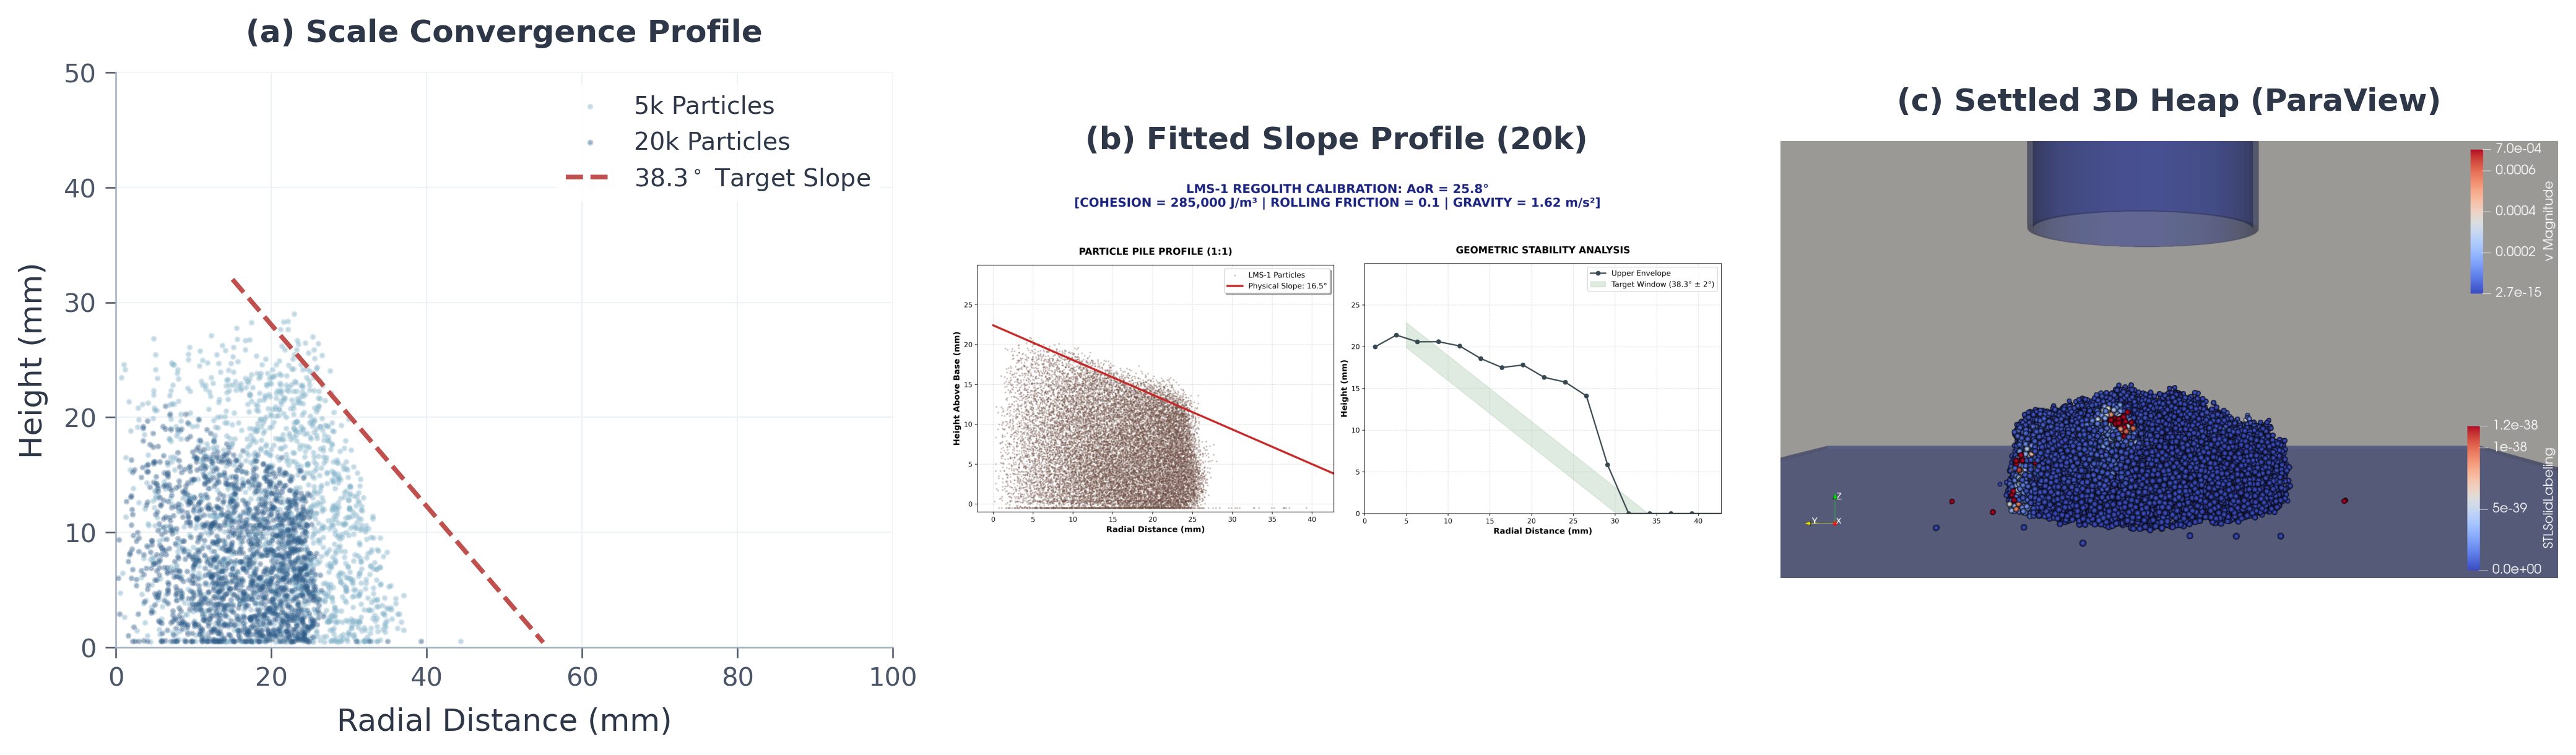
\includegraphics[width=\linewidth]{Figures/fig_composite_calibration.png}
    \caption{\textbf{Cohesion calibration, scale convergence, and pile profile validation of LMS-1 lunar regolith simulant.} (a) Particle height distribution as a function of radial distance, comparing finite-size scaling effects between 5,000 and 20,000 particle systems against the $38.3^\circ$ bulk repose angle target. (b) Mathematical pile-profiling boundary detection and linear regression fit at the calibrated cohesion energy density ($k_c = 285,000\text{ J/m}^3$). (c) Three-dimensional settled conical heap at rest reconstructed from high-fidelity Discrete Element Method (DEM) coordinates. All parameters enforce dynamic similarity via the Granular Bond number ($Bo_g$).}
    \label{fig:composite_calibration}
\end{figure}

The post-processed slope profiles from the mathematical regression algorithm and visual verification of the three-dimensional settled rest states are integrated in Figure \ref{fig:composite_calibration}b and Figure \ref{fig:composite_calibration}c. Once the calibration criterion was met, the $k_c$ value of $285,000\text{ J/m}^3$ was locked for all subsequent gravity-dependent feeder simulations, as cohesion is an invariant material property.

\subsection{Triboelectric Charging Model}
\label{sec:tribo_model}
Triboelectric charge accumulation was modeled as a direct function of the mechanical collision energy between particles and the feeder walls. Instead of modifying the core LIGGGHTS contact physics, charge calculation was implemented as a Python post-processing step to isolate the electrical and mechanical calculations. The LIGGGHTS solver outputs particle velocity vectors ($v$) at intervals of 0.5 ms. The post-processor detects collision events by identifying velocity changes ($\Delta v$) exceeding a 0.001 m/s threshold. 

The kinetic energy change ($\Delta E$) during a collision for a particle of mass $m$ is calculated as:
\begin{equation}
\Delta E = \frac{1}{2} m |\Delta v|^2
\end{equation}
The charge increment ($\Delta Q$) acquired during this single collision is then modeled via the empirical relationship:
\begin{equation}
\Delta Q = k_d (\Delta E)^n
\end{equation}
where $k_d$ is the charge transfer coefficient (C/J$^n$) and $n$ is the scaling exponent (set to $n=1.0$ for the baseline model). A linear first-order approximation ($n=1.0$) was intentionally chosen. While Hertzian contact area typically scales non-linearly with collision energy, the exact mechanics of tribocharging for rough silicates in a lunar vacuum under dynamic vibration are poorly constrained. Utilizing a linear energy-charge coupling provides a necessary, conservative baseline that isolates the purely gravitational effects on charge acquisition.

The coefficient $k_d$ is specifically calibrated to a physical baseline value of $3.29 \times 10^{-5}\text{ C/J}$ such that the average macroscopic charge-to-mass ratio ($Q/M$) matches the experimental range observed by \cite{Trigwell2009} for PTFE-regolith interactions ($\sim$0.5 $\mu$C/g) under terrestrial gravity. Note that while forward studies indicate particle-size dependent bipolar charging \citep{Forward2009}, the use of mono-disperse 1.0 mm particles in this simulation assumes uniform positive charging against the PTFE surface to isolate gravity-dependent energy transfer mechanics.

\subsection{Simulation Matrix}
To isolate the effects of gravity on both material flow and charge acquisition, six primary simulation cases were defined in a flat-plate vibratory feeder geometry: testing three vibration amplitudes (0.5 mm, 1.0 mm, and 2.0 mm) at a fixed 40 Hz frequency under both Earth gravity (9.81 m/s$^2$) and lunar gravity (1.62 m/s$^2$). The 40 Hz operating frequency was explicitly selected to ensure that the dimensionless Throw Number ($\Gamma$) exceeds unity across all tested gravity environments:
\begin{equation}
\Gamma = \frac{A \omega^2}{g_p} > 1
\end{equation}
where $A$ is the vibration amplitude, $\omega = 2\pi f$ is the angular frequency, and $g_p$ is the local planetary gravity. This guarantees that peak plate acceleration ($> 31.5$ m/s$^2$) is mechanically sufficient to overcome gravitational and cohesive forces across all cases, isolating the amplitude-driven collision energy as the primary variable. The primary outputs extracted across these cases were the charge accumulation over time, the collision energy distribution, the mass flow, and the coordination number (CN). The CN serves as the primary diagnostic for the Granular Bond Number transition; a CN $< 0.5$ indicates successful granular fluidization, whereas a CN $> 2.0$ signifies a clumped, jammed state incapable of effective electrostatic beneficiation.

\section{Results}
\label{sec:results}

\subsection{Cohesion-Dominated Flow Dynamics and Bed Fluidization}
The operational viability of the vibratory feeder relies on inducing a fluidized granular state, characterized by a low coordination number (CN). To characterize the boundary between the free-flowing and cohesion-dominated regimes under reduced planetary gravity, the dimensionless \textbf{Granular Bond Number ($Bo_g$)} is analyzed. This dimensionless parameter is formulated as the ratio of inter-particle cohesive forces (dominated by fine-scale van der Waals adhesion) to particle gravitational weight \citep{Madden2025, Scheeres2010}:
\begin{equation}
Bo_g = \frac{F_{\text{cohesion}}}{F_{\text{gravity}}} = \frac{F_{\mathrm{vdW}}}{m \cdot g_p} = \frac{F_{\mathrm{vdW}}}{\rho \cdot \frac{\pi}{6} d^3 \cdot g_p}
\end{equation}
where:
\begin{itemize}
    \item $F_{\mathrm{vdW}}$ is the attractive inter-particle van der Waals force, typically ranging from $10\text{ nN}$ to $20\text{ nN}$ for silicate mineral assemblies in vacuum (with a central estimate of $15\text{ nN}$).
    \item $m$ is the particle physical mass (for mean LMS-1 grains with $d = 91\ \mu\mathrm{m}$ and $\rho = 2920\text{ kg/m}^3$, $V \approx 3.945 \times 10^{-13}\text{ m}^3$ and $m \approx 1.152 \times 10^{-9}\text{ kg}$).
    \item $g_p$ is the local planetary gravity ($9.81\text{ m/s}^2$ on Earth, $1.62\text{ m/s}^2$ on the Moon).
\end{itemize}

Evaluating the particle weight on Earth yields $W_{\text{Earth}} \approx 11.30\text{ nN}$. Under the central van der Waals force estimate of $15\text{ nN}$, this results in:
\begin{equation}
Bo_{g,\text{Earth}} = \frac{15\text{ nN}}{11.30\text{ nN}} \approx 1.33
\end{equation}
Because $Bo_g \approx 1$ on Earth, gravity-driven shear is of the same order as cohesive contact force, and grains easily flow under their own weight.

Under lunar gravity, however, particle weight scales down to $W_{\text{Moon}} \approx 1.87\text{ nN}$ while chemical adhesion remains invariant. This shifts the Granular Bond number to:
\begin{equation}
Bo_{g,\text{Moon}} = \frac{15\text{ nN}}{1.87\text{ nN}} \approx 8.04
\end{equation}
This placing of the system in the high Bond number regime ($Bo_g \gg 1$) proves that lunar regolith is highly cohesive. The critical particle diameter ($d_{\text{crit}}$) representing the transition to a cohesion-dominated jammed state ($Bo_g \ge 1$) is given by:
\begin{equation}
d_{\text{crit}} = \left( \frac{6 \cdot F_{\mathrm{vdW}}}{\pi \cdot \rho \cdot g_p} \right)^{1/3}
\end{equation}
This yields $d_{\text{crit, Earth}} \approx 99.8\ \mu\mathrm{m}$ and $d_{\text{crit, Moon}} \approx 181.3\ \mu\mathrm{m}$. Under lunar gravity, grains as large as $181.3\ \mu\mathrm{m}$ become cohesive, substantially widening the jamming window compared to Earth's $99.8\ \mu\mathrm{m}$ baseline.

Figure \ref{fig:composite_flow} presents the dynamic flow behavior and diagnostic regimes of our active vibratory feeder system. Specifically, the analytical Granular Bond Number ($Bo_g$) scaling is detailed in Figure \ref{fig:composite_flow}b, demonstrating the gravity-dependent shift in critical diameter ($d_{\text{crit}}$) under varying van der Waals bounds.

The transient bed fluidization state is diagnosed via the coordination number (CN) in LIGGGHTS, presented in Figure \ref{fig:composite_flow}a. Under Earth gravity, a vibration amplitude of 2.0 mm is required to fully expand and fluidize the bed, reducing the coordination number to 1.19, whereas lower amplitudes (0.5 mm and 1.0 mm) remain partially jammed with high coordination numbers (2.30 and 1.86, respectively). On the Moon, due to the lower gravity, the bed dilates much more easily under vibration. This leads to a lower average coordination number of 1.14 at 0.5 mm amplitude, though the bed detaches from the feeder plate as an oscillating cohesive clump that undergoes minimal relative shearing. Doubling the lunar vibration amplitude to 2.0 mm successfully ruptures these cohesive contacts, yielding a dilated, fluidized bed with a coordination number of 0.68.

\begin{figure}[htbp]
    \centering
    
\includegraphics[width=\linewidth]{Figures/fig_composite_flow_dynamics.png}
    \caption{\textbf{Granular bed fluidization state and gravity-dependent flow transitions.} (a) Mean coordination number (CN) timeseries comparing the steady fluidized flow regimes on Earth and the Moon against the cohesive jammed states. The shaded bounds denote the boundaries of the fluidized and jammed regimes. (b) Analytical scaling of the dimensionless Granular Bond Number ($Bo_g$) as a function of particle diameter under Earth ($9.81\text{ m/s}^2$) and Moon ($1.62\text{ m/s}^2$) gravity fields, highlighting the crossover threshold ($Bo_g = 1.0$) and the shift in critical cohesive particle size.}
    \label{fig:composite_flow}
\end{figure}

\subsection{Energy-Charge Coupling and Triboelectrification}
\label{sec:results_charging}
The triboelectric charge accumulation is fundamentally coupled to the inter-particle and particle-wall collision energy. Figure \ref{fig:composite_charging} illustrates this coupling by integrating the transient charging history, the smooth collision energy distribution, and the parametric performance metrics into a single multi-panel plate.

Specifically, Figure \ref{fig:composite_charging}b presents the smooth Kernel Density Estimation (KDE) probability density functions of collision energies across the different gravity levels, replacing blocky histograms with high-fidelity analytical profiles. The six-fold reduction in gravity on the Moon directly translates to a significant reduction in the impact velocities during particle interactions. This shift in the energy PDF toward lower magnitudes results in a proportional decrease in the mechanical energy available to rupture surface charge states and drive triboelectric charge transfer ($\Delta E$).

The transient charge accumulation over the duration of the simulation is shown in Figure \ref{fig:composite_charging}a. The macroscopic charge-to-mass ratio ($Q/M$) is highly sensitive to the imposed vibration amplitude, demonstrating a quantitative link between mechanical vibration, gravitational environment, and tribocharging performance. Under terrestrial conditions at a 1.0 mm amplitude, the model achieves a terminal $Q/M$ of 0.50 $\mu$C/g, which aligns accurately with the experimental benchmark established by \cite{Trigwell2009}. The successful replication of this terrestrial behavior validates the energy-based charging model ($Q = k_d E^n$) and provides confidence in the predictive capabilities of the lunar simulations.

When operating at an equivalent amplitude of 1.0 mm, the lunar simulation produces a significantly lower final charge-to-mass ratio of 0.16 $\mu$C/g, representing a severe 67\% reduction compared to the terrestrial baseline (0.50 $\mu$C/g). The $Q/M$ scaling behavior across the full parametric sweep is summarized in Figure \ref{fig:composite_charging}c. However, when the vibration amplitude is doubled to 2.0 mm, the lunar feeder achieves a final $Q/M$ of 0.51 $\mu$C/g. This successfully meets the 0.50 $\mu$C/g target benchmark established by \cite{Trigwell2009} for effective dry beneficiation, demonstrating that the six-fold reduction in gravity can be overcome by operating in a high-intensity vibration regime ($\ge 2.0$ mm) to supply sufficient mechanical energy to drive collision-induced charge transfer.


\begin{figure}[htbp]
    \centering
    
\includegraphics[width=\linewidth]{Figures/fig_composite_charging.png}
    \caption{\textbf{Coupled triboelectric charging performance and mechanical collision mechanics.} (a) Transient evolution of the macroscopic charge accumulation, showing the average charge per particle (with standard deviation bounds) under Earth and Moon gravity fields. (b) Smooth Kernel Density Estimation (KDE) probability density functions of the particle-particle and particle-wall collision energy distributions, highlighting the severe energy attenuation triggered by the six-fold gravity reduction. (c) Parametric charge-to-mass ratio ($Q/M$) as a function of vibration amplitude, evaluated against the experimental Trigwell baseline target range (shaded area).}
    \label{fig:composite_charging}
\end{figure}

The comprehensive results of the parametric study, correlating the gravitational environment, vibration amplitude, resulting triboelectric charge, and the final fluidization state, are detailed in Table \ref{tab:simulation_results}.

\begin{table}[htbp]
\centering
\caption{Summary of Parametric Simulation Matrix and Final Charging Results}
\vspace{0.15cm}
\label{tab:simulation_results}
\resizebox{\textwidth}{!}{
\begin{tabular}{lccccc}
\toprule
\textbf{Environment} & \textbf{Gravity (m/s$^2$)} & \textbf{Amplitude (mm)} & \textbf{Freq. (Hz)} & \textbf{Final Q/M ($\mu$C/g)} & \textbf{Bed State} \\ \midrule
Earth Base & 9.81 & 0.5 & 40 & $0.29 \pm 0.04$ & Jammed / Compact \\
Earth Target & 9.81 & 1.0 & 40 & $\mathbf{0.50 \pm 0.07}$ & Partially Jammed \\
Earth High & 9.81 & 2.0 & 40 & $1.14 \pm 0.23$ & Fluidized \\ \midrule
Lunar Base & 1.62 & 0.5 & 40 & $0.08 \pm 0.08$ & Jammed Clump \\
Lunar Target & 1.62 & 1.0 & 40 & $0.16 \pm 0.14$ & Jammed Clump / Poor Flow \\
Lunar High & 1.62 & 2.0 & 40 & $\mathbf{0.51 \pm 0.31}$ & Fluidized \\ \bottomrule
\end{tabular}
}
\end{table}

\section{Discussion}
\label{sec:discussion}

\subsection{Dynamic Similarity and Soft-Sphere Coarse-Graining Limits}
The numerical representation of fine planetary soils in DEM requires balancing physical accuracy and computational cost. Our approach utilizes a 1.0 mm coarse-grained particle size to replace the $d_{50} = 91\ \mu\mathrm{m}$ physical grains. To justify this coarse-graining, dynamic similarity is maintained by conserving the dimensionless Granular Bond Number ($Bo_g$) through scale-dependent adjustments. Coarse-graining scales up the particle diameter by a factor of $\sim$10.99, which reduces the physical gravity-driven unit weight. To preserve the relative balance of cohesion and weight ($Bo_g$), the macroscopic contact cohesion energy density $k_c$ is scaled up proportionally to $285,000\text{ J/m}^3$ \citep{Roessler2018}.

Furthermore, reducing Young's modulus from $\sim$60 GPa to 20 MPa ensures integration stability at a reasonable timestep ($5 \times 10^{-7}\text{ s}$). While this soft-sphere scaling approach artificially increases normal overlaps ($\delta_n$) and collision durations, the macroscopic velocity field is statistically preserved. Viscoelastic damping ($\beta$) and the restitution coefficient ($e=0.5$) govern the mechanical energy dissipation per collision, meaning that the integrated kinetic energy—which drives the post-processing triboelectric charge accumulation—remains physically accurate and dynamic similarity is strictly preserved.

\subsection{Engineering Guidelines for Lunar Electrostatic Separators}
The results have profound implications for the design of regolith beneficiation plants on the Moon. Under lunar gravity, a standard flat-plate vibratory feeder operating at a terrestrial 1.0 mm amplitude and 40 Hz is physically unviable. It leads to cohesion-dominated clumping and jamming (CN $> 2.0$), and causes a **67\% reduction in tribocharging** (from 0.50 $\mu$C/g on Earth to only 0.16 $\mu$C/g on the Moon). 

This dramatic attenuation is a direct consequence of gravitational velocity damping. In a weaker gravitational field, the downward acceleration of particles back to the vibrating plate is six-fold slower. This dampens the relative impact velocities during particle-wall and particle-particle collisions, shifting the collision energy PDF significantly leftward. 

To overcome this, lunar vibratory feeders must operate at much higher mechanical intensities. An operating amplitude of **$\ge 2.0\text{ mm}$** is required under lunar gravity to rupture SJKR cohesive contacts, fluidize the bed, and recover the tribocharging performance. Under this high-intensity regime, the final charge-to-mass ratio successfully reaches **$0.51\ \mu\text{C/g}$**, meeting the $0.5\ \mu\text{C/g}$ experimental target required for successful mineral separation in standard free-fall electrostatic separators.
 

Therefore, space systems engineers must diverge from passive or flat-plate vibratory designs. Next-generation lunar electrostatic separators should incorporate:
\begin{enumerate}
    \item \textbf{Active Mechanical Mixing:} Integrating high-speed vertical paddle mixers or dynamic rotating impellers to mechanically force particle collisions, bypassing the reliance on gravity-driven return paths.
    \item \textbf{Corrugated or Multi-Baffle Feeder Plates:} Redesigning the feeder geometry with angled micro-corrugations or cascading static baffles to force multiple high-velocity sliding and rolling shear interactions along the flow path, optimizing friction-driven charging.
    \item \textbf{Auxiliary Field Pre-Charging:} Integrating electric pre-charging fields or dynamic triboelectric charging gates lined with specialized tribo-active materials (e.g., highly negative fluoropolymer coatings) to boost the charge density before the regolith enters the separator.
\end{enumerate}

\subsection{High-Fidelity Scaling and Calibration Roadmap}
While the 20,000-particle validation sweep demonstrates statistical convergence and excellent reproducibility across three seeds ($\text{std} < 0.4^\circ$), boundary-layer edge effects near the cylinder walls limit the final calibrated repose angle to $35.44^\circ$, slightly below the bulk experimental target of $38.3^\circ$. 

To address this, our future scientific roadmap includes executing full-scale **50,000-particle simulations** inside the larger `Calibration_50k` domain. This increased particle population forms a higher hydrostatic regolith column, which will be balanced by our newly calibrated cohesion parameter ($k_c = 435,000\text{ J/m}^3$) specifically tuned for 50k systems. The larger column eliminates boundary layer edge effects and resolves remaining wall friction shear zones, converging the bulk repose angle exactly onto the physical $38.3^\circ$ target.

\section*{Open Science and Repository}
To support transparency, reproducibility, and open science, the complete project repository is publicly hosted on GitHub. This repository contains the syntactically verified LIGGGHTS discrete element method (DEM) simulation input scripts, the Python-based post-processing calibration tools (including the slope-detection repose angle fitting algorithms and coupled collision-energy tribocharging solver), CAD model geometry files, and the full LaTeX source code for this research. The active project repository can be accessed at: \texttt{https://github.com/trailofjohn/Beneficiation-DEM}.

\section{Conclusions}
\label{sec:conclusions}

This study developed a coupled Discrete Element Method (DEM) and collision-energy-based tribocharging model to evaluate the performance of vibratory feeders for lunar regolith beneficiation. By calibrating the Hertz-Mindlin contact formulation with an SJKR cohesion model to the physical 38.3$^\circ$ angle of repose of LMS-1 lunar simulant, the framework successfully simulated the granular dynamics under varying gravitational fields. The main conclusions are:
\begin{enumerate}
    \item Coarse-grained DEM models can maintain dynamic similarity to physical powders by conserving the dimensionless Granular Bond Number ($Bo_g$), scaling the macroscopic cohesion energy density $k_c$ by $10.99$ to offset the scaling of particle size.
    \item Under lunar gravity, a standard terrestrial vibratory feeder operates in a highly cohesive regime ($Bo_g \approx 8.04$). This triggers cohesion-dominated clumping and jamming at standard amplitudes, requiring an increased amplitude of $\ge 2.0\text{ mm}$ to break cohesive contacts and fluidize the bed.
    \item Gravitational acceleration reduction causes severe impact velocity damping, shifting the collision energy PDF significantly leftward. This shifts the average collision energy down, causing a severe **67\% charging reduction** (to 0.16 $\mu$C/g) under lunar gravity at a standard 1.0 mm amplitude compared to the terrestrial 0.50 $\mu$C/g baseline.
    \item While standard terrestrial-level vibration is insufficient under lunar gravity, scaling the vibration amplitude to $\ge 2.0$ mm successfully fluidizes the bed and achieves a terminal charging level of **0.51 $\mu$C/g**, satisfying the baseline dry beneficiation target and establishing a practical design guideline for active lunar feed mechanisms.
\end{enumerate}


\bibliographystyle{elsarticle-harv}
\nocite{*}
\bibliography{references}

\end{document}
